%!TEX root = ../template.tex
%%%%%%%%%%%%%%%%%%%%%%%%%%%%%%%%%%%%%%%%%%%%%%%%%%%%%%%%%%%%%%%%%%%%
%% chapter3.tex
%% NOVA thesis document file
%%
%% Chapter with a short latex tutorial and examples
%%%%%%%%%%%%%%%%%%%%%%%%%%%%%%%%%%%%%%%%%%%%%%%%%%%%%%%%%%%%%%%%%%%%

\typeout{NT FILE chapter3.tex}%

\makeatletter
\newcommand{\ntifpkgloaded}{%
  \@ifpackageloaded%
}
\makeatother


\chapter{Elaboration}
\label{cha:elaboration}

In this chapter, we give a conceptial overview of the proposed solution. We begin by presenting the general overview of the system model and the design goals in Section~\ref{sec:system_model}, followed by a more tecnical description of the techniques and tecnologies used in the implementation of the prototype in Section~\ref{sec:prototype_guidelines}. Finally, we present how we intend to test and validate our implementation in Section~\ref{sec:validation}.

\section{System Model}
\label{sec:system_model}

\subsection{Initial System Model Approach}\label{subsec:initial_system_model_approach}

As shown in Section~\ref{sec:problem}, Tor is a widely used network for anonymous communication. However, it has some vulnerabilities that can be exploited by attackers to de-anonymize users, such as traffic analysis attacks. Several techniques have been proposed to mitigate these attacks, such as k-anonymity, but they lack formal guarantees of privacy and are almost based on practical validations, which in real-world applications might vary. In this context, we proposed a new approach to enhance the privacy of Tor users by integrating a differential privacy mechanisms in Tor relays and on the Client side. Our approach aims to develop a Differential Private Scheduler similiar to KIST (Section~\ref{subsubsec:kist}) that will be responsible for adding noise to the traffic flows in order to protect the privacy of users. 
The Tor scheduler handles two buffers, input and output. The first receives the cells and the second sends them. Between these two buffers, the circuit queue is responsible for managing the cells that are being processed. 

\begin{figure}
    \centering
    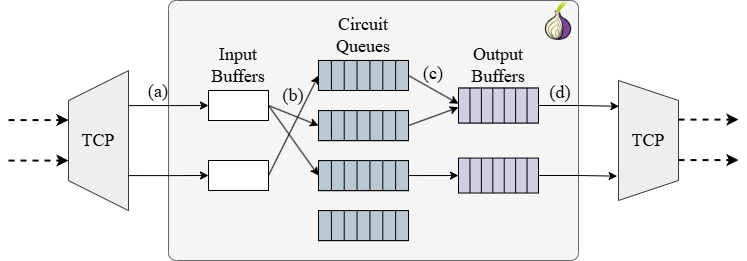
\includegraphics[width=0.8\textwidth]{Chapters/Figures/Fig1.png}
    \caption{Tor Relay Internal Architeture}
    \label{fig:initial_system_model}
\end{figure}

The Tor Relay Internal Architeture is shown in Figure~\ref{fig:initial_system_model}. 
When a relay receives a TCP packet, the kernel processes them and delivers to Tor (Figure~\ref{fig:initial_system_model}(a)).
Upon receiving the entire packet, Tor onion-encrypts it and the cell is enqueued into the circuit queue (Figure~\ref{fig:initial_system_model}(b)). 
Each circuit queue represents a circuit that the relay maintains. In this example, this relay is part of 4 circuits, each with a different circuit queue. Nonetheless, this does not mean that the relay must have an input buffer for each circuit, since a single TCP connection may be part of multiple circuits. 
The scheduler is responsible for selecting a cell from the circuit queue to be sent to the output buffer (Figure~\ref{fig:initial_system_model}(c)).
Finally, when the relay's output buffer contains sufficient data to form a TLS packet, the data is sent via TCP connection (Figure~\ref{fig:initial_system_model}(d))~\cite{KIST, EWMA}.

\subsection{Our System Model Approach}\label{subsec:our_system_model_approach}

The Tor Relay described in Figure~\ref{fig:initial_system_model} represents a simple relay. Our goal is to provide formal guarantees of privacy to users of Tor network whilst maintaing practical levels of performance. To achiave this goal, we propose a new approach to enhance the privacy of Tor users by integrating a differential privacy mechanisms in Tor relays and on the Client side. 
Our approach aims to develop an differential private mechanisms, called \textit{Differential Privacy Scheduler Compenent}, that is responsible for adding noise to the traffic flows based on several parameters in order to protect the privacy of users.  
\begin{figure}
    \centering
    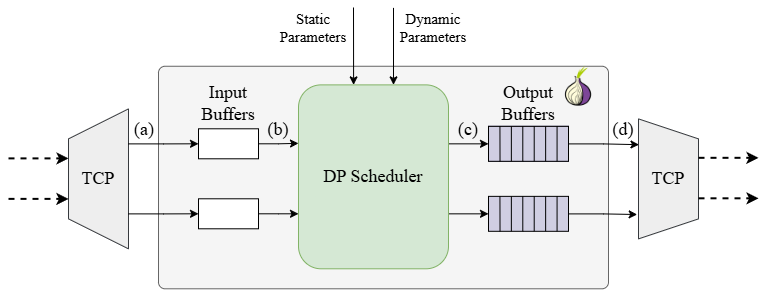
\includegraphics[width=0.8\textwidth]{Chapters/Figures/Fig2_dp.png}
    \caption{Enhanced Tor Relay with Differential Privacy  Scheduler Component}
    \label{fig:our_system_model}
\end{figure}
Figure~\ref{fig:our_system_model} illustrates the enhanced Tor Relay internal architeture with our Innobservability Scheduler Component. This component is responsible for adding noise and control to the traffic flow, focusing on improving the circuit queue scheduler algorithm. This component has a variable levels of performance and privacy, according to the parameters set by the relay or dynamically calculated.   

\subsection{Differential Privacy Scheduler}\label{subsec:differential_privacy_approach}

The Differential Privacy Scheduler, or DP Scheduler, is a component that maintains the circuit queues and is responsible for selecting the cells to be allocated in the output buffer, just like the vanilla Tor scheduler. In addition, the DP scheduler uses a set of parameters to allow customization on the level of privacy and performance. These parameteres can be split into two categories: static, or configuration, and dynamic.
\begin{itemize}
  \item \textit{Static Parameters}: These parameters are set by the relay operator. One of these parameters is the queue size, called privacy window, which determines the number of cells that the DP Scheduler will consider to execute the differential private algorithm and, therefore, apply noise into this window and subsequently into the traffic. Another static parameter is the privacy parameter, often denoted by $\epsilon$, which determines the level of privacy that the DP Scheduler will provide. Our work aims to provide a confirgurable file that allows the relay operator to set these parameters before running the relay.
  \item \textit{Dynamic Parameters}: These parameters are calculated by the DP Scheduler based on the current state of the relay and the network. An example of dynamic parameter is the 
\end{itemize}

This component represents a sutle change in the Tor Relay internal architeture, but we believe that it can significantly improve users' privacy, based on the differential privacy formal guarantees that we aim to provide.

\section{Prototype Guidelines}\label{sec:prototype_guidelines}

In order to implement the proposed solution, we have 2 main approaches: the Tor approach and the Mirace approach. The Tor approach consists of modifying the Tor source code to include the Differential Privacy Scheduler Component. The Mirace approach consists of creating a new relay that will be responsible for adding noise to the traffic flows.

\subsection{The Tor Approach}\label{subsec:tor_approach}

\subsection{The Mirace Approach}\label{subsec:mirace_approach}

\section{Validation}
\label{sec:validation}

\subsection{Performance Measurements}\label{subsec:performance_measurements}

\subsection{Innobservability Measurements}\label{subsec:innobservability_measurements}

\section{Summary}
\label{sec:elaboration_summary}


